\documentclass[conference]{IEEEtran}
\IEEEoverridecommandlockouts
% The preceding line is only needed to identify funding in the first footnote. If that is unneeded, please comment it out.
\usepackage{cite}
\usepackage{amsmath,amssymb,amsfonts}
\usepackage{algorithmic}
\usepackage{graphicx}
\usepackage{textcomp}
\usepackage{xcolor}
\def\BibTeX{{\rm B\kern-.05em{\sc i\kern-.025em b}\kern-.08em
    T\kern-.1667em\lower.7ex\hbox{E}\kern-.125emX}}
\begin{document}

\title{Distributed Multiplayer Video Game}

\author{\IEEEauthorblockN{Ryan Wickman}
\IEEEauthorblockA{\textit{University of Memphis} \\
Memphis, USA \\
rwickman@memphis.edu}
}

\maketitle

\begin{abstract}
This is a write up for a project done in my COMP-7212 class.
It specifies the implmentation details, designs, and hurdles of creating a distributed multiplayer game from scratch.
\end{abstract}

\section{Introduction}
In this section I will provide a brief overview of the project and its implementation details.

\subsection{Goal}
The goal of this project initially was to create a full peer-to-peer multiplayer video game, of which I got pretty close to accomplishing.
However, due to time constraints, I switched the scope of it to mainly focus on the matchmaking server, demo video game, and client-side communication with the matchmaking server.
Thus my goal was updated to establish a good baseline matchmaking server and communication pipeline so that players of a video game could use to find and join a game session.
Although my goal was updated, I still designed the areas I was not able to fully implement (e.g., the peer-to-peer in game communication).

\subsection{Overview}
In this project, I worked on a few major components of what makes up a mutliplayer video game.
What this entailed was making a way for users to send information amongst one another once in the game, a matchmaking server users could use to connect to a game, and the game itself.
I decided to use a peer-to-peer architecture for the in game communication for users. 
While this may cause more latency than a dedicated, centralized server, it scales better and is more cost efficent for myself.
In this, one player is chosen to host the game and acts like the server.
The rest of the players will communicate through the host user as if it was a dedicated server itself.
They will use UDP to communicate as the game is a real-time application and is thus time sensitive.
On the other hand, the matchmaking server will be centralized as there needs to be a single point for all users to connect and express interest in finding a game session to join.
The users will use TCP, as opposed to UDP, to connect to the matchmaking server as reliable data transfer is important for finding and joining a game.

The game was developed using the Unity game engine and programed in C\# .
It is has a main menu that users can use to find a game through the matchamking server or connect to a game directly by using an IP address of the host.
The actual gameplay is a first-person sword fighting game.
While I have a good working example for these components, this is far from the final product of what it will eventually be.
Thus throughout this paper I will provide incite to where I beleive the application could be improved or expanded on as well.

\section{Matchmaking Server}
The majority of the time I spent on this project was focused on the matchmaking server.
It ended up having a lot more moving components than I first anticipated.
I used C++ to code everything, CMake to manage the build procces, and Boost.Asio to provide the asynchronous networking capability.
The server is made up of a few parts main moving parts: matchmaking server interface, TCPConnection, and game queue.
The rest of the parts are used in conjunction with these main parts of which I will explain in the following subsections.

\subsection{Packet}
In the exchanging of information between independent applications there needs to be a uniform way to pass and read message in support of interoperability. 
Such a requirement requires an agreement between the communicating applications such as them both following a specific protocol.
Due to this, I created my own packet types that the front-end video game programmed in C\# can use to communicate with the back-end matchmaking server programmed in C++.
The packets carry data that is created by one side and  consumed by the other side.
The data in the packets are in JSON data format, which uses key-value pairs.
This has to be serialized before it is sent over the network and deserialized when it arrives to its destination.
The reason I chose this data format is because there are libraries in both C\# and C++ that support the usage of JSON and it rather easy to use.

The packets themselves were designed to be lightweight and easily extensible.
There are a many different packet types I created throughout this project; I will give a description of all of them later on in this section.
They all inherit from the parent class Packet and have the naming scheme of "\textlangle packet type\textrangle Packet".
The Packet class has member variables for the header length, maximum body length, body length, a char array to store the data, and a packet type.
The header length is the fixed amount of bytes contained in the header.
The maximum body length is the upper limit for the amount of bytes that can be contained in  a packet.
The body length is the amount of bytes contained in the body.
The data char array is where the header and body are actually stored and what is actually sent over the network when communicating.
The header is the first 8 character of the data array and it contains the body length.
The reason for having a header store this information is because the body of a packet differs between packet types.
Furthermore, it allows for variable length packets which thus provides more granularity of the data sent and reduces wasted bandwidth consumption.
The body of the packet is what contains the actual payload of the packet: the serialized JSON data.
This JSON data differs between packet types; however, all of them contain the key-value pair for the packet type.

The Packet class also has member functions to access its protected members, to decode and encode the header, to decode the body, and to encode both the header at once body.
The functions to access the protected members include data(), body(), length(), body\textunderscore length(), and packet\textunderscore type().
All of these are self-explanitory given their names.
The only interesting one is Packet::body() which returns data\textunderscore + header\textunderscore length.
The reason for doing this is because of pointer arithmetic in C++, this will return a pointer to the first char in the body.

The function Packet::set\textunderscore body\textunderscore length is used to set the body length of the packet, but will cap it at the maximum body length if an attempt is made to exceed this upper limit.
The function Packet::encode\textunderscore header() is used to serialize the packet header.
First, it creates a temporary char array called header of size header length + 1.
Then, It then writes the body length to this char array,
Finally, it copies the bytes in this char array to the data member variable.

The function Packet::decode\textunderscore header is what is used to decode the serialized header that is stored in the member data array.
It return a boolean indicated if the it was successful in decoding the header.
First, it creates a temporary char array called header of size header length + 1.
Then, it copies the first 8 bytes of the data array into the header array.
Next, it sets the body length to the integer represented by this array of chars.
Finally, if the body length is greater than the max body length it sets body length equal to 0 and returns false.
If the body length is less than or equal to the max body length it returns true.

As you may notice I have yet to explain the functions for decoding and encoding the body.
This is because they are pure virtual as to enforce the children classes to provide their own implementation to encode and decode the body. 
The reason for doing this is because the information contained in the body of a packet differs between packet types.
Now I shall explore the classes that inherit from Packet.

The class FindPacket is what is used when a user wants to join a game.
It contains two additional members variables for a unique identifier for the client and the game type the user wants to join.
It also has additional member function for accessing the members and the implementation details for encode and decode\textunderscore body.
The FindGamePacket::encode function is used to serialize the member variables of the class and the header so it can be sent over the network.
First, it creates a JSON data type.
I am using a library called nlohmann to achieve this.\cite{b1}
Second, It sets the key-value pairs for the packet type, user ID, and game type.
Third, it serializes the JSON data and stores it in a string called find\textunderscore game\textunderscore str.
Fourth, it calls set\textunderscore body\textunderscore length with the size of find\textunderscore game\textunderscore str as its argument.
Fifth, it encodes the header.
Finally, it copies find\textunderscore game\textunderscore str to the body of the packet.

The  FindGamePacket::decode\textunderscore body function is what is used to decode the body for use of the receiver of the packet.
First, it deserializes the data by parsing it into a JSON object called find\textunderscore game\textunderscore json.
Second, it sets the member variables to the values of find\textunderscore game\textunderscore json.

For this instance I gave an explanation of Packet::encode and Packet::decode\textunderscore body; however. for the rest of the packet types I will not give one as the implementation is extremely similar.
The only differences include getting and setting the unique member variables for each packet types.


The JoinPacket class is provided by a host a game session to client users whom want to join the game. 
It contains information required by the users to join said game.
The two member variables it contains is the IP address of the host and the PID of the game session.

The HostPacket class is used by the GameQueue to tell a user to host a game.
The only member variable it contains is the game type the user needs to create a session of.

The AckPacket class is used to keep the TCP connection alive while the users is waiting to join or host a game.
I will give more details to this later and why it is necessary in the TCPConnection section.
It contains member variables for the ack type,
This ack type is of type AckType which is an enum defined in the ack\textunderscore type.hpp file.
It currently only has two possible values None and Error.
The ack\textunderscore type.hpp file also includes a class called ack\textunderscore error.
This is used when the value of ack type is set to Error.

Nonetheless that finishes the discussion on the different packet types and their individual usage.
I will go into more detail later on how each one is used in the matchmaking server setting.


\subsection{Mathmaking Server Interface}
This is the point in which the user will first connect to the server.
The server is listening on a specified port and accepts incoming requests when the arrive. 
It asynchronously accepts the requests then initiates a callback that handles setting up the TCP socket to the client.
This allows for multiple users to connect to the server at once. 
The socket is constructed by initializing a TCPConnection object that will handle the rest of the users communication to find a game.
While I did consider creating a new thread for each connection, I did not due to time constraints and not wanting to deal with the complexity of adding multithreading such as locking resources, race conditions, ect..
When I update this application in the future I will potentially add this feature.

\subsection{TCPConnection}
The bulk of my time that I spent on the matchmaking server was on the TCPConnection class.
This is due to many factors such as redesigns, updating call sequences, callbacks, and simply just the overall complexity of this component.
The job of this component pertains  to handling the communication with the user that allows them to connect to a game session.
This is done through a series of callback functions that create asynchronous read and write operations.
In the other sections I explained each member of the class in no particular order, however in this section I will explain them as I go through the process of how it works.

The first thing that occurs is the TCPConnection object is instantiated after a user connects to the server.
The TCPConnection is created by factory method aptly named create.
This function has two parameters for a boost::asio::io\textunderscore context reference called io\textunderscore context and a GameQueueManager reference called game\textunderscore queue\textunderscore manager.
It calls the private constructor for TCPConnection and returns a shared pointer to the created object.
The parameter  io\textunderscore context is used to create an I/O object of type boost::asio::ip::tcp::socket called socket\textunderscore .
The member variable socket\textunderscore is used throughout the TCPConnection object to perform the asynchronous write and read operations.
The other parameter, the GameQueueManager reference, is used to populate a member variable game\textunderscore queue\textunderscore manager\textunderscore .
The GameQueueManager is used to geta game queue of specific type to put the client in.
I will go into the details of this later.

After the TCPConnection object is created, its start function is called.
The function TCPConnection::start only does one thing: calls TCPConnection::do\textunderscore read\textunderscore find\textunderscore game\textunderscore header.

The function TCPConnection::do\textunderscore read\textunderscore find\textunderscore game\textunderscore header is used to read the header of the FindGamePacket that will be sent by the user.
First, it will set the local variable self to the result of the call share\textunderscore from\textunderscore this() which returns a shared\textunderscore ptr\textlangle TCPConnection\textrangle object that shares ownership of *this.
Second, it will start the asynchronous operation by calling boost::asio::async\textunderscore read.
The arguments to this function include the TCP socket object, the buffer to read the data into, anda callback function to be fired once the read operation completes.
The buffer is created from the data char array of a member variable of type FindGamePacket called find\textunderscore game\textunderscore packet and its header length, 8 bytes.
The callback function is a lambda function that captures this and the self variable created earlier and takes in parameters that are populated by Boost.Asio when the read operation completes.
These parameters are boost::system::error\textunderscore code ec and std::size\textunderscore t length.
The ec variable indicated whether an error occurred and the length is how much data was read, in this case it should be 8 bytes unless an error occurs.
Now after this operation is requested, the TCP connection stays alive until this operation is complete.
The reason for this being that shared pointer to *this is passed to the callback function of the asynchronous read.
The TCPConnection object cannot be destroyed until the last shared pointer reference is destroyed.
When the header of the FindGamePacket header is read, the callback is fired.
The callback first checks if an error has not occurred and if it can successfully decode the FindGamePacket header.
If both of these are true, then TCPConnection::do\textunderscore read\textunderscore find\textunderscore game\textunderscore body is called.
If not, then the TCP socket is closed.

The function TCPConnection::do\textunderscore read\textunderscore find\textunderscore game\textunderscore body reads the body of the FindGamePacket from the client.
It is similar to what occurs in TCPConnection::do\textunderscore read\textunderscore find\textunderscore game\textunderscore body so I will skip some of the details.
Once the body is read the callback function for this asynchronous read operation commences.
First, it decodes the body of the packet.
Second, it uses the game\textunderscore queue\textunderscore manager\textunderscore  member variable to get the game queue for the game type specified in the FindGamePacket object.
Third, if both the previous steps are successful, it will create a User object using the user ID from the FindGamePacket instance, the IP address from the socket, TCPConnection::host\textunderscore game, and TCPConnection::join\textunderscore game. 
Fourth, it will push this created User instance on the queue.
Fifth, it will call TCPConnection::do\textunderscore read\textunderscore ack\textunderscore header.

Once the queue is ready to start the game, there at two main code paths the TCPConnection will envoke: either it will be host that will create a game session or act as a client and join the game craeted by a different user.
Both of these can be seen in Figure 1 and Figure 2.

If it is the host, it will send the HostPacket to the client.
The client will first send back a AckPacket and then a JoinPacket.
This JoinPacket will be sent to all others User who will join the game.
The distribution of the JoinPacket is handled by the GameQueue when TCPConnection calls the start callback on the User.

If it is not the host, the TCPConnection will just send the JoinPacket to the client and close the connection.

\begin{figure}[h]
\centerline{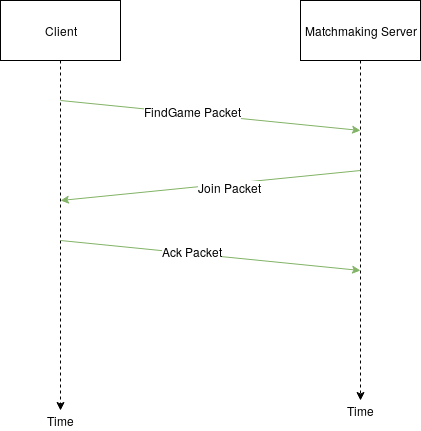
\includegraphics[width=\linewidth, height=6cm]{figures/ClientCommunication.png}}
\caption{An example of communication that will occur when a user will act as a client in the game session }
\label{fig}
\end{figure}

\begin{figure}[h]
\centerline{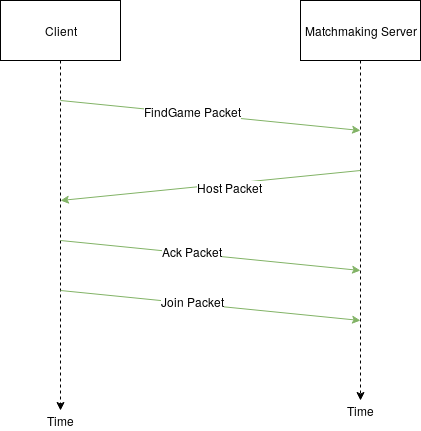
\includegraphics[width=\linewidth, height=6cm]{figures/HostCommunication.png}}
\caption{An example of communication that will occur when a user will act as a client in the game session. }
\label{fig}
\end{figure}

\subsection{Game Queue}
Before a user is able to join a game session, they need to wait their turn so that everyone who came in before them has the chance to join a game. 
This is why I went with a FIFO data structure such as a queue to implement this feature. 
However, in a video game with multiple game types, a user may only want to join a specific one.
Thus, it would not make sense for users looking for different game types to be in the same queue.
My solution to these requirements is to have a GameQueue superclass that is inherited from by all queues handling the users of a specific game type. \par
This class has members variables for the queue that stores weak pointers to Users, an unordered user map, the game type of this queue, the minimum and maximum size of a game session, the current queue size, and a boolean flag for if a game is currently getting prepared.
The queue is a std::queue that simply stores std::weak\textunderscore ptr\textlangle User\textrangle types. The reason it stores this type and not a User directly is because a connection may get dropped while a user is in queue.
If this occurs, then the queue will be able to correctly verify this by checking if the User object the pointer points to is expired before it uses it.
The user map is used to keep track of the amount of times a user has been added to a queue.
This, however, is not to prevent duplicate entries in the queue, but to make sure the user’s place in the queue is updated.
For example, once a game is initiated and a user is popped from the queue it will need to verify its count is equal to 1 to add it the game session.
If its count in this maps is greater than 1, then it will decrement this count and go on to the next user in the queue.
If its count is 0 then it assumed this user was erased from the queue and it does nothing.
You might be thinking what is the point of all this and why not just remove the user from the queue when a duplicate is detected or if an erase is called?
Initially I did think about doing this.
However, for many reasons I decided against it.
For one, on average it takes O(1) time to look up an element in a map, while it takes O(n) to erase an element from a queue.
So it is faster.
Albeit, it does add extra space complexity of O(n) so there is a bit of a trade off.
Additionally, in the future when introduce multithreading to this application, race conditions will begin to be an issue.
If I was to erase an element from the queue while concurrently trying to pop an element out undefined behavior may occur.
To prevent this, the queue would have to be locked until the erase finishes.
Instead a simple update to the user map will not effect the queue operation.
The worst case scenario is a user is added to a game before they should be because they were removed from the queue before the user map could update their count.
This of course could also be fixed by locking the queue, but would take less time on average due to the smaller time complexity.
The current queue size is used to keep track of the amount of unique users in the queue.
This will always be less than or equal to the actual queue size as there could be duplicate users in the queue.
The game type of the game queue is represented as an enum value.
I have a file, game\textunderscore type.hpp, specifying all the possible game types as an enum.

There are also several member functions in the GameQueue class: push, pop, erase, prepare\textunderscore game, and start\textunderscore game.
They are all pure virtual function as it is up to the inheriting class to define their behavior.
This of course makes the GameQueue class abstract, and thus I only have the GameQueue header and not associated cpp implementation file.
Currently, due to time constraints,  I only have one game type called deathmatch.
Its class is aptly named DeathmatchGameQueue.
All future GameQueue children will follow this naming convention of "\textlangle game type\textrangle GameQueue".
This class has same members as the GameQueue superclass, albeit, with its own unique implementation of member functions of which I will explain in depth.

The DeathmatchGameQueue::push function has a single parameter of type std::shared\textunderscore ptr\textlangle User\textrangle \& aptly named user.
This is what is being requested to be added to the queue.
First, it will see if the user has already been added to the queue by checking if the user ID is in the user map.
If it is not, it is inserted in the user map with a count of 1 and the queue size is incremented.
If it is in the queue, but its count is less than 0, meaning its been erased from the queue but not yet popped off, then it will set its count to 1 and increment the queue size.
If it is already in the queue and its count is greater than 1 then it will only increment its count. 
After checking its count, the user is added to the queue.
Finally, if this added user made the queue large enough to start a game and a game is already not getting prepared it will call DeathmatchGameQueue::prepare\textunderscore game.

The DeathmatchGameQueue::pop function is a little more complicated than I initially hoped.
This is due to the unforeseen complexity of having duplicates in the queue and the potential of having a user whose connection is closed in the queue.
When the pop function is called, it will first check if the current queue size is less than or equal to 0.
If it is, it will return a default weak\textunderscore ptr that points at nothing, so just null.
Then, if queue size is greater than 0, it will keep trying to get a user off the queue until it find a user that still has an active connection.
If no such user is found it will return weak\textunderscore ptr\textlangle User\textrangle ().
Now, once a user is found, it will check if the user is duplicated in the queue.
If it is, it will pop out users out of the queue until it finds one that is not duplicated.
When duplicates are removed in this way, their count is decremented.
Finally, once a nonduplicated, alive user is found it will erase it from the user map, decrement the queue size, and return a weak pointer to the user.

The DeathmatchGameQueue::erase function is rather simple.
It first checks if the user is in the user map.
If it is, then it is removed from the user map and the queue size is decremented.
This operation is again O(1) on average rather than O(n) and thus the erase function becomes O(1) on average.

The DeathmatchGameQueue::prepare\textunderscore game function is what I said earlier is called once the queue reaches a certain minimum size.
Firstly, it will set a boolean flag to true to indicate a game is getting prepared.
Secondly, the user in the front is popped off the queue.
Thirdly, it will call the host\textunderscore callback function on the user passing in a reference to DeathmatchGameQueue::start\textunderscore queue function and the game type of this queue.

The DeathmatchGameQueue::star\textunderscore game function is used as a callback that is fired by the TCPConnection object of a host of a game once it is ready for users to join the game it is hosting.
It has a single parameter for a JoinPacket.
First, the packet is encoded, which serializes the packet to get ready to be sent over the wire to the user.
Then, the it will enter in a while loop that will continue as long as a maximum amount of users have been added or the queue is empty.
Next, inside this loop a user is popped off this queue, the current game size is incremented, and the join\textunderscore callback on the user is called with the JoinPacket object passed as an argument.
Finally, the preparing game flag is set to false.

Now that wraps up the implementation and design of the game queue.

\subsection{User}
The User class was created so that an item could be added to the game queue that is representative of a unique user.
Additionally, it contains smart pointers that contain references for callback functions that are used to allow the user to join or host a game.
Originally I planned on having a reference to the TCPConnection object in the User class.
However, the problem to this is it would create a circular dependency with the GameQueue class.
This is because the GameQueue class includes the header for the User class declarations and the TCPConnection includes the header for the GameQueue class declarations.
So, instead the User has reference to the functions "TCPConnection::host\textunderscore game and "TCPConnection::host\textunderscore game" to prevent such a circular dependency, but still have the necessary functionality.
This also provides more control for the TCPConnection to decide and handle what exact functions gets called.
In the future, this may prove helpful if I require different users to behave differently when joining or hosting a game.
One such instance would be if a private game is being created where only select users are able to join.
This join callback could provide additional authentication statements to verify a user can join a game before making a failed attempt and the TCPConnection closing thinking the user found a game.

\section{The Video Game}
In this section I will give the implementation details of the video game itself, the client-side matchmaking, and provide the design for the in game peer-to-peer communication.
\subsection{Gameplay}
The video game that the matchmaking system will support is a simple 3D first-person sword fighting game.
It was created using the Unity game engine and programmed in C\#.
Note in the previous sections I used  client and user interchangeably, as those are both common terms to describe the person asking for a service or interacting with a service in the networking field.
In the video game development field it is more appropriate to describe this person as a player.
There are a few different inputs a player perform to interact with the environment and other players.
You can move your player character in the game by using the arrows keys or WASD and use the mouse to look around or change your direction while moving.
You can also attack/swing the sword by clicking the left mouse button.

The way the player moves is by applying a force on the Rigidbody component attached the the player GameObject.
The Rigidbody component is something built into Unity that allows for adding physical force to an object rather easy, as opposed to building an entire psychics system yourself.
In the game, force is applies based on the input and speed of the character.
The direction the player wants to move is given by the arrows keys.
This is restricted to be in the x and z axis only, as the y axis corresponds to the character floating up or down.
This direction vector is then normalized to be a unit vector and multiplied by the character’s speed and Time.delataTime (e.g., direction * speed * Time.deltaTime).
The speed is a scalar value, not a vector, to denote the magnitude the player should move in a particular direction.
Time.deletaTime is the completion time in seconds since the last frame.\cite{b2}
It is used to keep the movement of the character frame independent and instead time dependent.
The reason this occurs is because the time in between frames is not always constant.

As written a second ago, the player can use the mouse to change the direction the character is looking.
This is done by changing the position and rotation of the Camera GameObject
The Camera is what  updates what the player sees on their physical screen.
At the beginning of the game, the Camera’s position is subtracted by the player character’s position and stored in a Vector3 variable called offset.
Then every frame, assume there are roughly 30 or 60 frames per second, the Camera’s position is set to the player character’s position plus this offset.
The math for doing this is rather simple: say A is the Camera’s position, B is the character’s position and C is the offset then A - B = C and B + C= A.
However, in the actually implementation I added linear interpolation to this expression as well to create a small delay between the movement of the character’s position and the Camera following.
So, how about the Camera’s rotation?
For example, how does the player look up and down in game?
The mouse x input is set as the yaw and the mouse y input is set as the pitch.
This pitch is clamped to a range of angles [-60, 50] to prevent the player from flipping the Camera upside down (e.g., if you were change pitch 180 degrees from its normal rotation range).

The character is able to left click to attack with there attached sword.
The swords has an attached collider, but it does not detect collisions.
Instead it is trigger collider, it detects when another collider, such as an enemy’s collider, enters.
The trigger collider is only activated once the player attacks and is deactivated once the attack is done.
This is to prevent damage being cause be just touching another character with the sword as opposed to attacking.
If this occurs, damage is inflicted to the enemy.
The enemy character can only be damaged once per attack.
This is enforced by keeping a HashSet that is used to identify if a character was already damaged in this attack.
It is reset (i.e., set to an empty HashSet) at the end of the character’s attack.
There is a delay between the the players ability to attack as to reduce the spamming of attacking.

Each character has a fixed amount of health.
When damage is inflicted, the health is reduced by the amount the sword inflicted.
If a character’s health is less than or equal to 0 then the character’s GameObject is destroyed (i.e., deleted from memory).

\subsection{Client-Side Matchmaking}
Although the video game has a lot of moving components that must interact with one another, is still just one machine doing all the processing.
Thus, multiplayer capability needs to be added to introduce the distributed system aspect.
In previous sections I described how the Matchmaking server looks from the server-side, I will now explain the client-side.
Similarly to the server-side, the client-side performs a series of asynchronous calls to get the user into a game session.

I created a basic main menu in Unity with the capability to find a game by simply clicking the find game button.
That is all the player sees so distribution transparency is present in this regard.
After the button is clicked a TCP socket and an asynchronous connect is started.
Currently, the IP address is fixed for the server, but in the future it will use a hostname and then resolve it to a IP address as to provide replication and relocation transparency.
Once the client is connected, the connect callback is called.
The connect callback calls another method called SendFindGame.
The SendFindGame method creates a FindGamePacket and sends it through the newly established connection.
So, how am I sending a FindGamePacket when it is programmed in C++ and this is in C\#?
Simple, just creating a JSON object that has the same key-value pairs and serializing it.
Once FindGamePackt is successfully sent, the callback handler of this send is fired and calls ReceiveHostOrJoin.
The method ReceiveHostOrJoin asynchronously reads the next packet.
In its callback, the data of the packet is passed.
If the packet type is a JoinPacket, an AckPacket is sent to the server then the client attempts to join the game session.
If the packet type is a HostPacket, then a AckPacket is sent to the server,  the game is created, then the JoinPacket is asynchronously sent back to the server.

\subsection{In Game Communication}
Once the players are actually in the game session, one player will act as the server and the rest will act as the clients.
This is a peer-to-peer system that allows for scalability and is cheap on my end as I will not have to pay for a dedicated server.
However this can impose higher latency on the players and may affect their experience.
Thus, in the future this may change depending on the player’s feedback of the system.

They will all communicate using UDP as this a real time application and is time sensitive.
Also, some lose of packets is tolerable.
For example, if a different player’s character walks to a new location in a frame and the packet is dropped this isn’t a game breaking error.
It is only micromential change to the game state and should not have serious repercussions as there are 30 to 60 frames per second.
The only effect this would have is the player movement would not look as smooth as if all the packets were sent.
As long as majority of the packet make it through then a few dropped packets should not have a huge effect on the overall gameplay.
Albeit, there may be times when some reliable data transfer is required.
This will be done on demand and be limited to when it is only necessary such as when a player is joining a game or critical information about the game state needs to be received by all clients.
Also note that I did not get around to implementing this part, unlike all the rest of the components and sections, so for now this is merely an idea based on what I have studied from other similar systems.

When a player creates a game session it will act as the host and the server for the game.
For another player to join, they will have to send a request the game’s host.
If the host (i.e., server) accepts, then the player may join the game.
There many cases when the server will decline the client request such as when it is private game, the game session is full, or the game requires authentication and the client did not have the correct authorization credentials.
Once the player is in the game, all current players will receive a notice that a new player has joined.
This packet will need to have reliable data transfer as it could cause serious problems if some players are not visible to everyone.
When a player receives this notice, it will create a GameObject for this player in its local environment.
This GameObject will be updated every time its associated client performs some type of action.
When a user does perform an action it will go through the server who will then distribute the action to all active clients.


However, instead of everyone communicating through the host in a star topology, they could communicate amongst one another in mesh topology.
Of course this would add extra complexity to the entire system.
It could potentially reduce the overall latency time as it will be decentralized and not rely entirely one the bottleneck for the host.
The host could be given the job of only updating the players when someone else joins, a new game is starting, and other simple game manager tasks
The player could then communicate with one another when they update an perform an action.
This could also be proximity based (i.e., only other character within a certain distance will receive a player action update.)

Nonetheless, I will need to do a lot of research in to find the best solution for the in game communication.

\section{Conclusion}
\subsection{Redesign}
At first I had trouble keeping the socket alive.
There were no outstanding read or write operations so it would automatically cancel close the socket without finishing the sequence of actions to get a user to join a game. 
My first solution to this problem resulted from looking through the boost asio documentation and discovering that a socket stays open as long as there is a shared\textunderscore ptr\textlangle T\textrangle object is still referencing the object.
So, I created a connection lock object called ConnectionLock that had a member varaible boost::shared\textunderscore ptr\textlangle TCPConnection\textrangle con.
The problem with this solution, however, is that the ConnectionLock instance must explicitly dereference the TCPConnection by setting con = nullptr.
This led to problems of making sure every code path that could throw an error or is done communicating must release this lock.
If not, the socket associated with the TCPConnection would never get closed resulting in a memory leak. 
Due to this being prone to error, I redesigned how to keep the socket alive through using the AckPacket.

\subsection{Future Work}
I plan to continue working on this project in the future.
I will expand open the current system and had ton more features.
\begin{itemize}
	\item Give the game queue the ability to start multiple games at a time
	\item Introduce multithreading to the matchmaking server
	\item Enforce timeouts for read and writes
	\item Finish implementing peer-to-peer in game UDP communications
\end{itemize}

\subsection{Final Thought}
Throughout this project I was able to gain a lot of experience in understanding the foundations on how distributed systems work.
I was able to implement communications that utilize interoperability through the packets.
I gained more experience in asynchronous communication with the server-side matchmaking and the client-side game.
I was also introduced with many challenges I did not initially think would spark up such as  keeping the TCP connection alive while waiting on the queue to fire a callback.
The repository for the matchmaking server can be found at https://github.com/rwickman/Matchmaking-Server.
You can find most of the code is under the server/ directory.
Also, the demo game can be found at https://github.com/rwickman/Distributed-Systems-Project.
The code is under Assets/Scripts/.
The reason I separated the repositories is because I plan on making matchmaking server extensible to other games besides just the one I created for this project.
Nonetheless, feel free to ask me an questions about any think at all.



\begin{thebibliography}{00}
\bibitem{b1} Nlohmann Json. (n.d.). Retrieved from https://github.com/nlohmann/json
\bibitem{b2} Time.deltaTime. (n.d.). Retrieved from https://docs.unity3d.com/ScriptReference/Time-deltaTime.html 
\end{thebibliography}
\vspace{12pt}

\end{document}
